\documentclass[aspectratio=169]{beamer}
\usepackage{graphicx} % Required for inserting images

\usepackage{transparent}
\usepackage{eso-pic}



\usetheme{Berlin}
\usecolortheme{beetle}



\setbeamercovered{transparent}

\usepackage{subcaption}
\usepackage{float}
\usepackage{subcaption}
\usepackage{pdflscape}
\usepackage{enumitem}
\usepackage{pifont}
\usepackage{parskip}
\setlength{\parskip}{5mm}
\usepackage{blindtext}
\usepackage[spanish,mexico]{babel}
\usepackage[normalem]{ulem}
%\usepackage{xcolor}
\usepackage{ragged2e}
\usepackage{multicol}
\usepackage{amsmath,amsthm,amssymb}
\usepackage{verbatim}
\usepackage{listings}

\usepackage{tcolorbox}
\usepackage{hyperref}
\usepackage{transparent}
\usepackage{eso-pic}
\hypersetup{colorlinks=true, linkcolor=magenta, urlcolor=orange, citecolor=orange}

%\usepackage{biblatex}
%\usepackage[backend=biber,citestyle=authoryear,style=apa]

\title[\insertframenumber/\inserttotalframenumber] {Los componentes de una computadora}
\author {Martínez Flores Jonathan\inst{1}\and Aquino Sumuano Jorge Carlos\inst{1} \and Macías Vargas Isaac Yair\inst{1}} 

\date{September 2024}

\setbeamertemplate{background}{
{\transparent{0.05}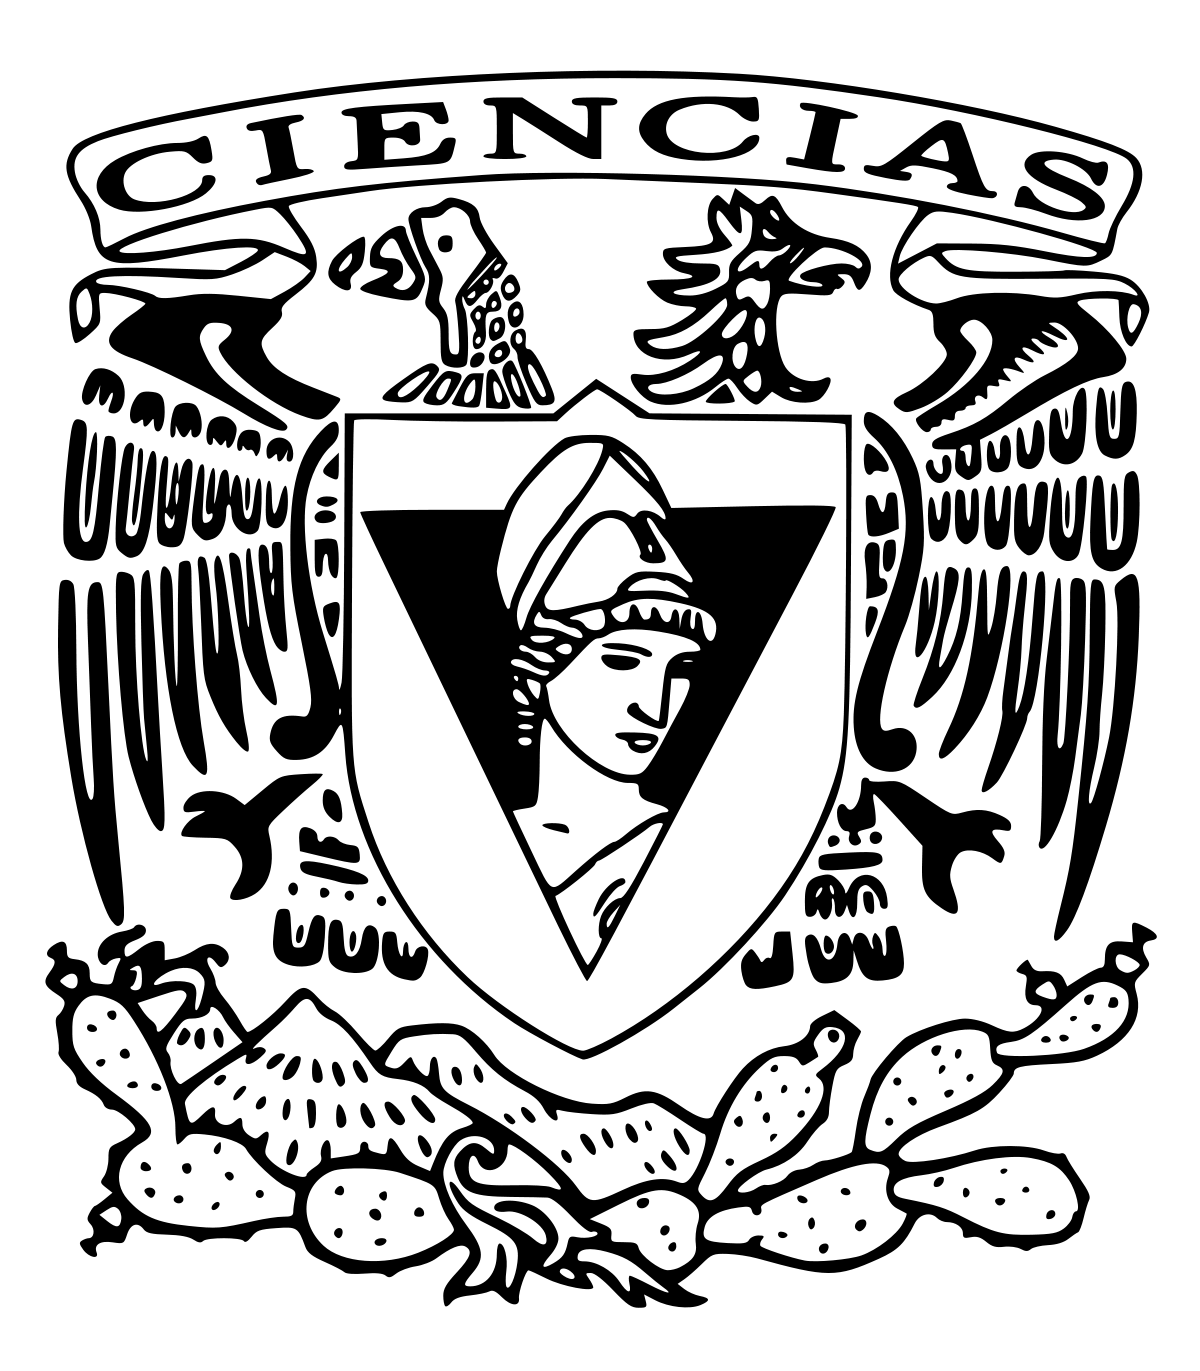
\includegraphics[width=1.0\paperwidth,height=1.0\paperheight]{escudo_fciencias.png}}
}

\AtBeginSection[]
{
\begin{frame}{Beamer}
\frametitle{Indice general}
 \tableofcontents{currentsection}   
\end{frame}
}

\AtBeginSection[]
{


}






\institute[]
{ 
 \inst{1}
 Facultad de ciencias \\ Universidad Nacional Autónoma de México

}

\setbeamertemplate{background}{\transparent{0.5}}





\begin{document}

\begin{frame}[plain]
\titlepage
    \begin{center}
        \includegraphics[scale=0.1]{UNAM.png}
        \hspace{5cm}\includegraphics[scale=0.077]{Ciencias.png}
    \end{center}
\end{frame}

\begin{frame}{T}
    \frametitle{Indice General}
    \tableofcontents{currentsubsection}
\end{frame}




\section{Introducción}
\begin{frame}{La importancia de conocer tu computadora}
    Componentes:
    \begin{block}{bloque sencillo}
        Este es un bloque
        \begin{enumerate}
            \item Ejemplo
            \item 
        \end{enumerate}
    \end{block}
\end{frame}


\subsection{Almacenamiento}
\begin{frame}{CPU y sus características}
El CPU (Central Processing Unity) está compuesto por:
\begin{exampleblock}{bloque de ejemplos}
\begin{itemize}
    \item 
    \item 
    \item
\end{itemize}
\end{exampleblock}
\end{frame}

\begin{frame}{La RAM (Random Access Memory) Memoria de Acceso Aleatorio}

   ALERTA

    
\end{frame}

\begin{frame}{ROM (Read-Only-Memory) Memoria de solo lectura}
    
\end{frame}
\section{Almacenamiento}
\begin{frame}{Tarjetas Gráficas (GPU-Graphics Processing Unit}
    
\end{frame}
\section{Almnacenamiento}
\begin{frame}{Discos duros vs de estado sólido (HDD vs SSD}
    
\end{frame}
\section{Circuitos y sistemas}
\begin{frame} {Funcionamiento de la Motherboard y la BIOS}
    
\end{frame}
\section{Conclusiones}
\begin{frame}{Conclusiones}
    
\end{frame}




\section{bibliografia}

\begin{frame}{allowframebreaks}{Bibliografía}
 \begin{thebibliography}
\bibitem{1}
\bibitem{2}


     
 \end{thebibliography}   
\end{frame}

\end{document}